\section{The Large Hadron Collider}
\label{sec:LHC}

The LHC was approved in 1994 by the CERN Council and was designed to collide hadrons, either protons or heavy ions, at instantaneous luminosity up to $10^{34}cm^{-2}s^{-1}$ and center-of-mass energies up to $\sqrt{s} = 14$ TeV \cite{LHCMachine}. LHC, the most powerful particle accelerator, is the successor of the Large Electron Positron Collider (LEP), which collided electrons and positrons at center-of-mass energies up to $\sqrt{s} = 250$ GeV \cite{LEP}. LHC reuses the same tunnel system as LEP with a circumference of $27$ km and lies $50$ to $175$ meters underground at the French-Swiss border outside Geneva, Switzerland. 

The first run of the LHC, Run-1, started in $2010$ at a center-of-mass energy of $\sqrt{s} = 7$ TeV, which was later increased to $8$ TeV. Run-1 lasted until $2013$, after which LHC was shut for two years of planned upgrades to enhance the accelerator and the detectors. LHC resumed its operation for Run-2 from $2015$ to $2018$ at the center-of-mass energy of $\sqrt{s} = 13$ TeV. The data collected during the Run-2 period is analyzed for this thesis. 

Accelerating the proton to the desired high center-of-mass energy is a multi-step process shown schematically in figure \ref{fig:ProtonAcc}. First, the protons are created from hydrogen gas by removing the electrons through ionization with an intense electric field. A proton beam is then formed in LINAC 2 linear accelerator and injected into the circular PS Booster, which accelerates the $50$ MeV proton to energies of $1.4$ GeV \cite{LHCGuide}. The beams are then injected into the Proton Synchroton (PS), accelerating them to energies of $25$ GeV \cite{LHCGuide}. The proton beams are then injected into the Super Proton Synchroton (SPS) to further accelerate at $450$ GeV energies and injected into the main LHC rings. The two opposite proton beams reach the desired final energy of $6.5$ TeV using radio frequency (RF) acceleration cavities \cite{LHCGuide}. The accelerated proton beams are maintained for several hours of data-taking.

\begin{figure}
    \centering
    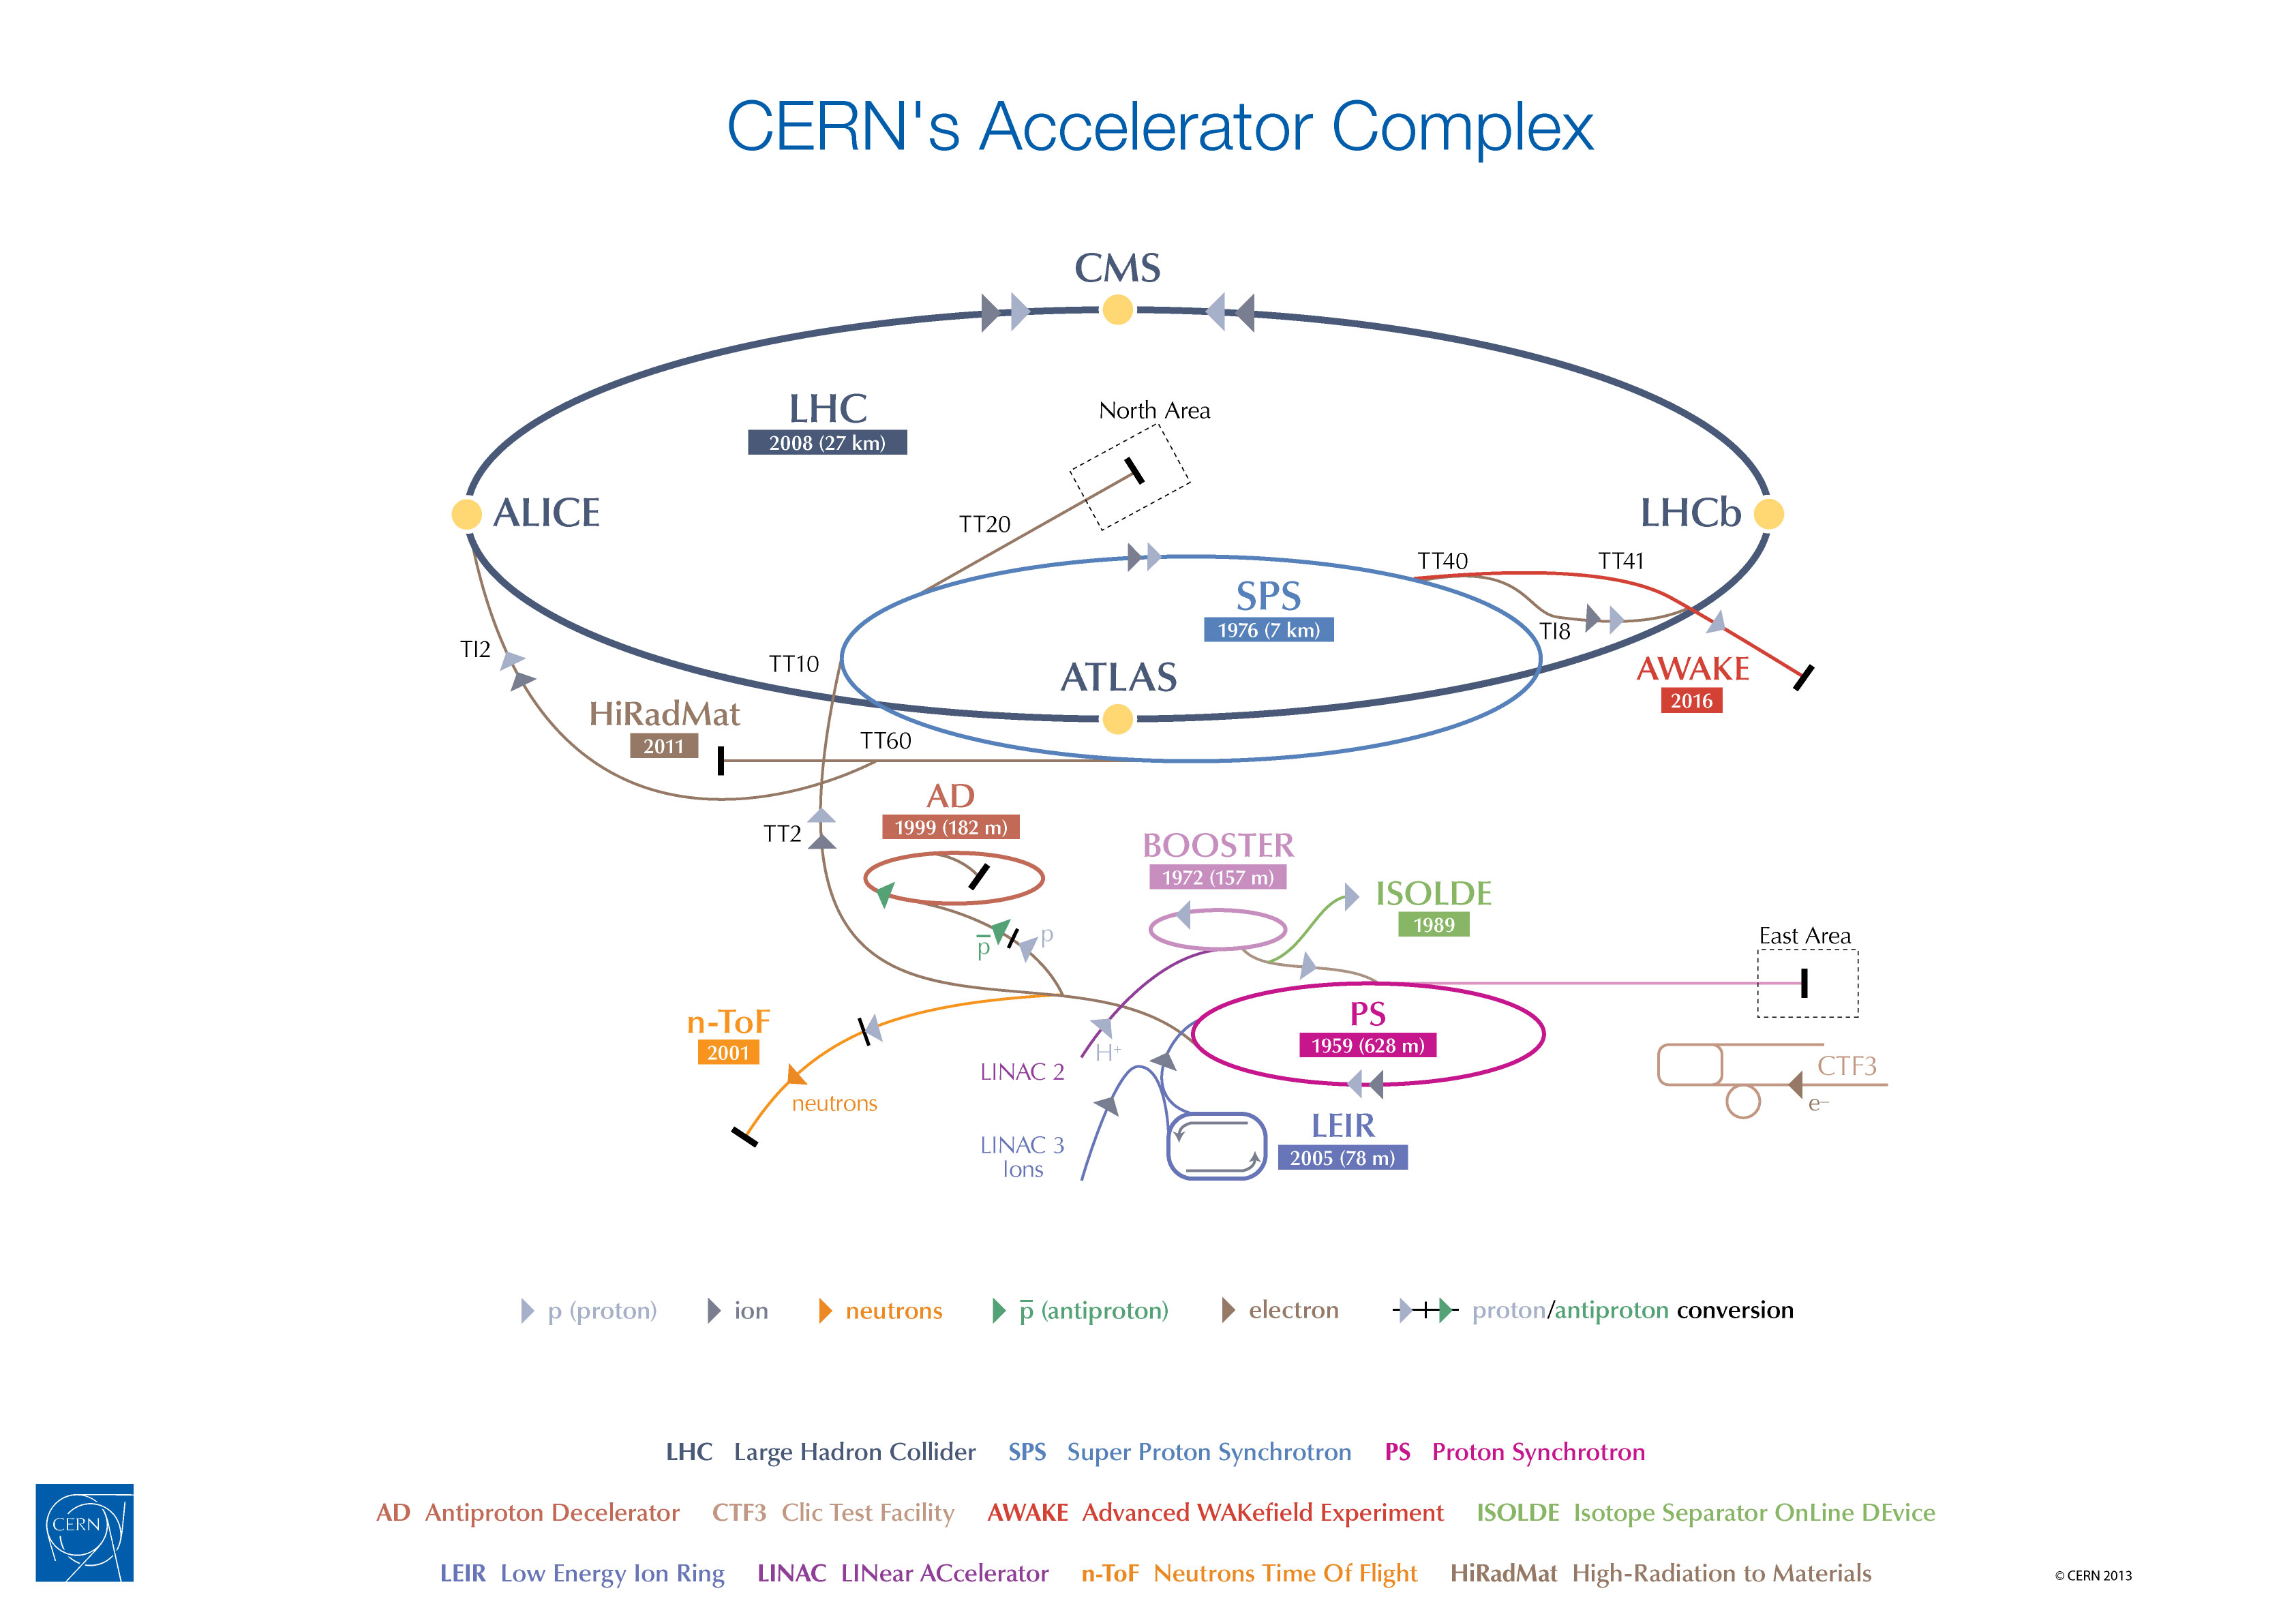
\includegraphics[width=.98\linewidth]{figures/LHC/ProtonAccelerator.jpeg}
    \caption{ A detailed layout of multiple-steps that goes into proton acceleration before entering the main ring \cite{ProtonAcclerator}.\label{fig:ProtonAcc}}
\end{figure}

The final RF accelerated proton beams are in evenly-spaced discrete bunches, each consisting of $10^{11}$ protons. The bunches are separated by $25$ ns spacing \cite{LHCGuide}. The proton beams are guided in the tunnel by a magnetic field using superconducting dipole and quadruplet magnets. The main LHC ring comprises $1232$ dipole magnets that provide a strong magnetic field of $8$T to bend the beams and about $392$ quadruplet magnets to focus the beams in the transverse plane \cite{LHCGuide}. The superconducting magnets are cooled down to $1.9$ K, which requires two vacuum systems to hold the cryomagnets and the helium distribution lines. To avoid unnecessary interactions, the beams are accelerated and maintained in an ultra-high vacuum of $10^{-13}$ atm \cite{LHCGuide}. 

The two opposite beam lines meet in four interaction points, thus, creating proton-proton collisions. The collisions are recorded by the four main detectors of LHC, ATLAS, CMS, LHCb, and ALICE. ATLAS and CMS are the two multipurpose experiments that perform new physics searches and precision SM measurements. ALICE experiment investigates the heavy-ion collisions and studies the quark-gluon plasma, whereas the LHCb experiment studies flavor physics \cite{LHCGuide}.